\section{Advanced Regression}

The chosen target variable is \texttt{averageRating}, which represents 
the average rating (on a 1--10 scale) assigned by IMDb users to each title. The exploratory 
data analysis showed that its distribution is approximately normal, 
with most titles concentrated in the range between 6 and 7. 
%For consistency with the classification task, the dataset was split into training 
%(70\%) and test (30\%) sets using the same stratification strategy.

\subsection{Random Forest Regression}
We applied the \textit{Random Forest Regression} algorithm on the task.
Before training the model, although not strictly necessary for tree-based models, 
we standardized the numerical features for consistency and transformed the categorical feature
\texttt{titleType} using \textit{One-Hot Encoding}.

The hyperparameters were optimized using \textit{RandomizedSearchCV} with 5-fold cross-validation, 
exploring different values for the number of trees (100, \textbf{200}, 300, 400, 500), 
the maximum depth (\textbf{None}, 10, 15, 20, 25, 30), 
the minimum number of samples required for a split (2, \textbf{5}, 10, 15) and for a leaf
(\textbf{1}, 2, 4, 6), and the number of features considered at each split (sqrt, \textbf{log2}). 
The best hyperparameters found are highlighted in bold. 
The \texttt{R\textsuperscript{2}} score was used as the evaluation metric during cross-validation.

 
The optimized Random Forest was first evaluated on the test set (results reported in Table~\ref{tab:rf_metrics}).
Subsequently, the model was retrained using only the 18 most important features identified through feature importance analysis.
Feature selection was guided by a cumulative importance plot, which showed that these 18 features accounted for over 90\% 
of the total importance, effectively reducing the dimensionality from the original 28 features without a significant loss in predictive performance.

\begin{table}[h]
\centering
\caption{Performance of the Random Forest Regressor on the test set 
(full model vs reduced features).}
\label{tab:rf_metrics}
\begin{tabular}{lccc}
\hline
\textbf{Model} & \textbf{MAE} & \textbf{MSE} & \textbf{R\textsuperscript{2}} \\
\hline
Random Forest (All Features) & 0.7536 & 1.0833 & 0.4033 \\
Random Forest (Top 18 Features) & 0.7550 & 1.0922 & 0.3984 \\
\hline
\end{tabular}
\end{table}

The results, reported in Table~\ref{tab:rf_metrics}, indicate that the Random Forest model achieves 
a mean absolute error below one point on the IMDb scale and explains around 40\% of the variance in the target variable. 
Notably, the model trained on only the top 18 features performs almost identically to the full-feature model 
(R\textsuperscript{2}: 0.3984 vs 0.4033), showing that 
predictive power is concentrated in a limited subset of variables. 
%These results represent solid performance, especially considering the subjective nature of ratings and the complexity of the domain.

Feature importance analysis further highlighted that the most influential predictors include both numerical variables,
such as \texttt{runtimeMinutes}, \texttt{startYear}, \texttt{ratingCount}, and \texttt{deltacredits},
and categorical variables derived from the encoding step, such as \texttt{titleType\_tvEpisode}, among others. 

\begin{figure}[h]
\centering
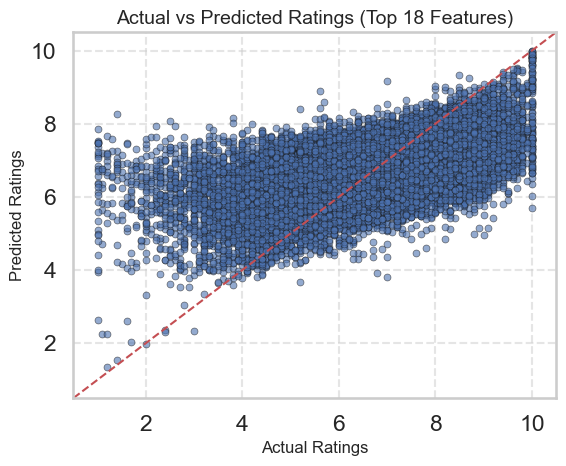
\includegraphics[width=0.7\textwidth]{plotsss/rf_top18_actual_vs_predicted.png} 
\caption{Actual vs Predicted \texttt{averageRating} for the Random Forest model trained on the top 18 features.}
\label{fig:rf_top18_actual_vs_predicted}
\end{figure}


The scatter plot in Figure~\ref{fig:rf_top18_actual_vs_predicted} shows that the predicted ratings roughly follow the trend of 
the actual ratings. Most predictions fall in the 6–7 range, consistent with the distribution of the target variable. 
While the model captures the general pattern, deviations occur, particularly at the extremes, which is consistent with the moderate R² of around 0.40. 
This indicates that the model explains a substantial portion of the variance, but there remains considerable unexplained variability.

% Questione cross validation ???